% =============================================================================
% supply-demand.tex — Classic supply/demand with a shifted demand curve
%
% Shows: upward-sloping supply S, two downward-sloping demands D1 and D2
% (D2 shifted right), with equilibria E1 and E2 marked.
%
% Compiles standalone via: xelatex supply-demand.tex
% =============================================================================

\documentclass[border=4pt]{standalone}
\usepackage{tikz}
\usetikzlibrary{arrows.meta}

\definecolor{supply}{HTML}{012169}
\definecolor{demand1}{HTML}{B23A48}
\definecolor{demand2}{HTML}{B9975B}
\definecolor{eq}{HTML}{1A1A1A}
\definecolor{axis}{HTML}{1A1A1A}

% -----------------------------------------------------------------------------
% Diagram: supply-demand with demand shift.
% Axes: Q on x, P on y. 1 cm = 1 unit.
% Supply line S: P = 0.5 + 0.5 Q → passes (0, 0.5) and (6, 3.5)
% Demand 1  D1: P = 4 - 0.5 Q    → passes (0, 4)  and (6, 1)
% Demand 2  D2: P = 5 - 0.5 Q    → passes (0, 5)  and (6, 2)
% Equilibria:
%   E1 = intersection(S, D1): 0.5 + 0.5Q = 4 - 0.5Q → Q = 3.5, P = 2.25
%   E2 = intersection(S, D2): 0.5 + 0.5Q = 5 - 0.5Q → Q = 4.5, P = 2.75
% Labels placed to the right/above of curves; no label in a curve sweep.
% -----------------------------------------------------------------------------

\begin{document}
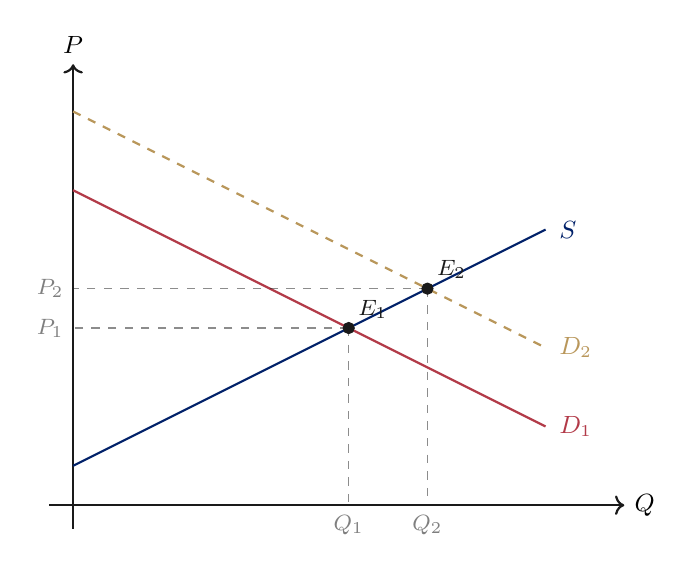
\begin{tikzpicture}
  % Axes
  \draw[->, thick, draw=axis] (-0.3, 0) -- (7, 0) node[right] {\small $Q$};
  \draw[->, thick, draw=axis] (0, -0.3) -- (0, 5.6) node[above] {\small $P$};

  % Supply
  \draw[thick, draw=supply] (0, 0.5) -- (6, 3.5);
  \node[right, supply, font=\small] at (6.05, 3.5) {$S$};

  % Demand 1
  \draw[thick, draw=demand1] (0, 4) -- (6, 1);
  \node[right, demand1, font=\small] at (6.05, 1) {$D_1$};

  % Demand 2 (shifted right / up)
  \draw[thick, dashed, draw=demand2] (0, 5) -- (6, 2);
  \node[right, demand2, font=\small] at (6.05, 2) {$D_2$};

  % Equilibria
  \filldraw[eq] (3.5, 2.25) circle (2pt) node[above right, font=\footnotesize] {$E_1$};
  \filldraw[eq] (4.5, 2.75) circle (2pt) node[above right, font=\footnotesize] {$E_2$};

  % Dashed guides
  \draw[dashed, draw=eq, opacity=0.5] (3.5, 2.25) -- (3.5, 0)
    node[below, font=\footnotesize] {$Q_1$};
  \draw[dashed, draw=eq, opacity=0.5] (4.5, 2.75) -- (4.5, 0)
    node[below, font=\footnotesize] {$Q_2$};
  \draw[dashed, draw=eq, opacity=0.5] (3.5, 2.25) -- (0, 2.25)
    node[left, font=\footnotesize] {$P_1$};
  \draw[dashed, draw=eq, opacity=0.5] (4.5, 2.75) -- (0, 2.75)
    node[left, font=\footnotesize] {$P_2$};
\end{tikzpicture}
\end{document}
